\PID 
Нека су познати импулсни одзиви \textit{LTI} система 
 $h_1 = h_1(t) = \ee^{-t} \uu(t)$, и $h_2 = h_2(t) = \ee^{-2t} \uu(t)$. Одредити 
импулсни одзив система у целини $h(t)$, у случају (а) серијске/редне/каскадне и (б) паралелне везе. 
\begin{figure}[ht!]
    \begin{subfigure}{0.5\textwidth}
        \centering
        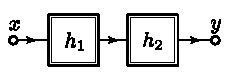
\includegraphics[page=1]{fig/ser_par.pdf}
        \caption{}
    \end{subfigure}
    %
    \begin{subfigure}{0.5\textwidth}
        \centering
        \includegraphics[page=2]{fig/ser_par.pdf}
        \caption{}
    \end{subfigure}
    \caption{}
\end{figure}

\RESENJE

За графичку представу структуре сложених система сачињених из више елементарних система примењују се тзв. \textit{стуртурни блок дијграми}
(или страћено, \textit{блок дијаграми}). У таквим дијаграмима, везе између блокова представљају појединачне сигнале а сами блокови системе.
Ток сигнала се може интерпретирати из контекста или се може експлицитно назначити стрелицама. Често коришћене ознаке система у оваквим дијаграмима 
представљене су у додатку \ref{a:blok}.

(а) Излаз првог система одређује се конволуцијом $x \ast h_1$, па тај сигнал онда представља побуду наредног (то је и смисао серијске везе система), 
па је укупан одзив $y = (x \ast h_1) \ast h_2$. Применом својства \textit{асоцијативности} операције конволуције (премештање заграда је 
могуће) се онда може писати 
$y =(x \ast h_1) \ast h_2 = x \ast \underbrace{( h_1 \ast h_2)}_{h}$. Укупан импулсни одзив целог система је
$h = h_1 \ast h_2$, па је на основу резултата задатка \ref{z:exp_konv} $h = (\ee^{-t} - \ee^{-2t}) \uu(t)$. 

(б) Излази појединачних систма су $x \ast h_1$ и $x \ast h_2$, па је због блока за сумирање импулсни одзив: 
$y = (x \ast h_1) + (x \ast h_2)$. На основу \textit{дистрибутивности} конволуције у односу на сабирање је онда 
$y = x \ast \underbrace{(h_1 + h_2)}_h$, односно $h = (\ee^{-t} + \ee^{-2t}) \uu(t)$.

Нагасимо на крају, још једном, да су општи резутлати овог задатка који су важни за наставак, да серијска веза два система даје конволуцију 
импулсних одзива, а да паралелна веза представља збир. Сликовита представа овог резултата представљена је на слици \ref{fig:\ID.1}.

Читаоцу се препоручује да размотри какво правило услед својства комутативности, и асоцијативности у односу на скаларно множење. 

\begin{figure}[ht!]
    \centering
    \includegraphics[page=3]{fig/ser_par.pdf}
    \caption{Уз резултат задатка. }
    \label{fig:\ID.1}
\end{figure}